% ═══════════════════════════════════════════════════════════════════════════════
% MODEL COMPARISON & STATISTICAL FIDELITY REPORT
% Aerospace Structural Design Dataset — L&T Technology Services
% ═══════════════════════════════════════════════════════════════════════════════
\documentclass[11pt, a4paper]{report}

\usepackage[utf8]{inputenc}
\usepackage[T1]{fontenc}
\usepackage{lmodern}
\usepackage[margin=2.2cm, top=2.5cm, bottom=2.5cm]{geometry}
\usepackage{graphicx}
\usepackage{booktabs}
\usepackage{longtable}
\usepackage{array}
\usepackage{xcolor}
\usepackage{hyperref}
\usepackage{fancyhdr}
\usepackage{titlesec}
\usepackage{caption}
\usepackage{subcaption}
\usepackage{amsmath}
\usepackage{multirow}
\usepackage{enumitem}
\usepackage{float}
\usepackage[most]{tcolorbox}
\usepackage{colortbl}
\usepackage{tabularx}
\usepackage{setspace}

% ── Colors ────────────────────────────────────────────────────────────────────
\definecolor{navy}{HTML}{1B2A4A}
\definecolor{teal}{HTML}{2EC4B6}
\definecolor{coral}{HTML}{E07A5F}
\definecolor{gold}{HTML}{F2CC8F}
\definecolor{lightbg}{HTML}{F7F9FC}
\definecolor{slate}{HTML}{6C7A89}
\definecolor{green}{HTML}{27AE60}
\definecolor{purple}{HTML}{7B68EE}

% Model colors
\definecolor{col-kde}{HTML}{2EC4B6}
\definecolor{col-gmm}{HTML}{4C9BE8}
\definecolor{col-cop}{HTML}{7B68EE}
\definecolor{col-td}{HTML}{27AE60}
\definecolor{col-tdp}{HTML}{1A7A4A}
\definecolor{col-mp}{HTML}{E8B84B}
\definecolor{col-tvae}{HTML}{E07A5F}
\definecolor{col-tvaep}{HTML}{C0392B}
\definecolor{col-ctgan}{HTML}{95A5A6}

% ── Styling ───────────────────────────────────────────────────────────────────
\hypersetup{colorlinks=true, linkcolor=navy, urlcolor=teal}
\setlength{\parindent}{0pt}
\setlength{\parskip}{6pt}
\onehalfspacing

\pagestyle{fancy}
\fancyhf{}
\fancyhead[L]{\footnotesize\textcolor{slate}{Model Comparison \& Statistical Fidelity Report}}
\fancyhead[R]{\footnotesize\textcolor{slate}{Aerospace Structural Design}}
\fancyfoot[C]{\thepage}
\renewcommand{\headrulewidth}{0.4pt}

\titleformat{\chapter}[display]
  {\normalfont\huge\bfseries\color{navy}}{\chaptertitlename\ \thechapter}{16pt}{\Huge}
\titlespacing*{\chapter}{0pt}{-20pt}{20pt}
\titleformat{\section}{\large\bfseries\color{navy}}{\thesection}{1em}{}
\titleformat{\subsection}{\normalsize\bfseries\color{navy!80}}{\thesubsection}{1em}{}

\newtcolorbox{insightbox}[1][]{
  colback=lightbg, colframe=teal, boxrule=0.8pt, arc=3pt,
  left=8pt, right=8pt, top=6pt, bottom=6pt, #1}

\newtcolorbox{patternbox}[1][]{
  colback=purple!5, colframe=purple, boxrule=0.8pt, arc=3pt,
  left=8pt, right=8pt, top=6pt, bottom=6pt,
  title={\textbf{Statistical Pattern}}, fonttitle=\color{navy}\bfseries, #1}

\newtcolorbox{findingbox}[1][]{
  colback=green!5, colframe=green!60!black, boxrule=0.8pt, arc=3pt,
  left=8pt, right=8pt, top=6pt, bottom=6pt,
  title={\textbf{Key Finding}}, fonttitle=\color{green!40!black}\bfseries, #1}

\newtcolorbox{modelbox}[2][]{
  colback=lightbg, colframe=#2, boxrule=1.2pt, arc=3pt,
  left=8pt, right=8pt, top=6pt, bottom=6pt, #1}

\graphicspath{{plots/}}

% ══════════════════════════════════════════════════════════════════════════════
\begin{document}

% ── Title Page ────────────────────────────────────────────────────────────────
\begin{titlepage}
\begin{center}
\vspace*{2cm}
{\Huge\bfseries\textcolor{navy}{Model Comparison \&}}\\[0.4cm]
{\Huge\bfseries\textcolor{navy}{Statistical Fidelity Report}}\\[0.9cm]
{\Large\textcolor{slate}{Aerospace Structural Design Dataset}}\\[0.3cm]
{\large\textcolor{slate}{Unified Evaluation of 9 Generative Models across 91 Configurations}}
\vspace{1.5cm}
\rule{0.65\textwidth}{1.5pt}\\[0.5cm]
{\large
\begin{tabular}{rl}
\textbf{Models:}        & 9 generative architectures (KDE, GMM, Copula, TabuDiff, \\
                        & TabuDiffPremium, MaskedPredictor, TVAE, TVAEPremium, CTGAN) \\[4pt]
\textbf{Datasets:}      & 91 synthetic configurations (3 seeds $\times$ up to 4 sizes per model) \\[4pt]
\textbf{Metrics:}       & 7 dimensions: fidelity, utility, privacy, correlation, physics \\[4pt]
\textbf{Raw data:}      & \texttt{data/model\_metrics\_aggregated.csv} (91 rows, 12 columns) \\[4pt]
\textbf{Date:}          & March 2026 \\
\end{tabular}}
\vspace{1.5cm}
\rule{0.65\textwidth}{1.5pt}
\vspace{2cm}
{\large Prepared for}\\[0.3cm]
{\Large\bfseries L\&T Technology Services}\\[1cm]
{\footnotesize\textcolor{slate}{Confidential. For authorised recipients only.}}
\end{center}
\end{titlepage}

\tableofcontents
\newpage

% ══════════════════════════════════════════════════════════════════════════════
\chapter{Executive Overview}
% ══════════════════════════════════════════════════════════════════════════════

\section{Study Design}

This report presents a unified evaluation of nine generative model architectures, each assessed across multiple dataset sizes and random seeds, yielding 91 synthetic datasets against the 300-row Aerospace Structural Design reference. The evaluation framework spans seven independent quality dimensions, enabling a multi-faceted comparison that resists reduction to a single ranking.

\begin{insightbox}
\textbf{Framing philosophy:} This report does not declare winners or losers. Each model architecture embodies a different set of inductive biases optimised for different statistical properties. The central finding is that the choice of generative model should be conditioned on which quality dimension matters most for the downstream application.
\end{insightbox}

\section{Evaluation Dimensions}

The seven metrics capture complementary aspects of synthetic data quality:

\begin{table}[H]
\centering
\caption{Evaluation metric definitions and interpretation direction.}
\label{tab:metrics}
\begin{tabularx}{\textwidth}{lXl}
\toprule
\textbf{Metric} & \textbf{What it measures} & \textbf{Direction} \\
\midrule
Physics Consistency      & Proportion of synthetic rows within physical bounds (schema + range) & Higher \\
Statistical Similarity   & Composite marginal distribution match (KS-based) & Higher \\
KS p-value (mean)        & Mean KS test p-value across 14 numeric features & Higher \\
KL Divergence            & Information-theoretic divergence from real distribution & Lower \\
ML Utility (TSTR)        & Random Forest macro-F1 trained on synthetic, tested on real & Higher \\
Privacy / Detection AUC  & AUC of discriminator trained to distinguish real vs synthetic & Higher (harder to detect) \\
Correlation Preservation & Closeness of synthetic vs real correlation matrix & Higher \\
\bottomrule
\end{tabularx}
\end{table}

\section{Headline Findings}

\begin{itemize}[itemsep=5pt]
\item \textbf{Statistical fidelity and composite score are near-synonymous.} Spearman correlations between Statistical Similarity / KL Divergence and the composite score both exceed $|r| = 0.97$, confirming that distribution-matching is the dominant quality signal in this evaluation.

\item \textbf{ML Utility is an orthogonal quality dimension.} With $r = 0.31$ against composite score, TSTR F1 provides genuinely independent information not captured by distribution matching alone.

\item \textbf{All nine models achieve near-perfect Physics Consistency.} Schema preservation ($r = 0.08$ with composite) is a solved problem across all architectures, confirming robust bound and schema adherence universally.

\item \textbf{Scale consistently improves all models.} Every architecture shows monotonic improvement in composite score as dataset size increases from 300 to 5{,}000 rows, with the magnitude of improvement varying by model class.
\end{itemize}


% ══════════════════════════════════════════════════════════════════════════════
\chapter{Composite Score Overview}
% ══════════════════════════════════════════════════════════════════════════════

\begin{figure}[H]
\centering
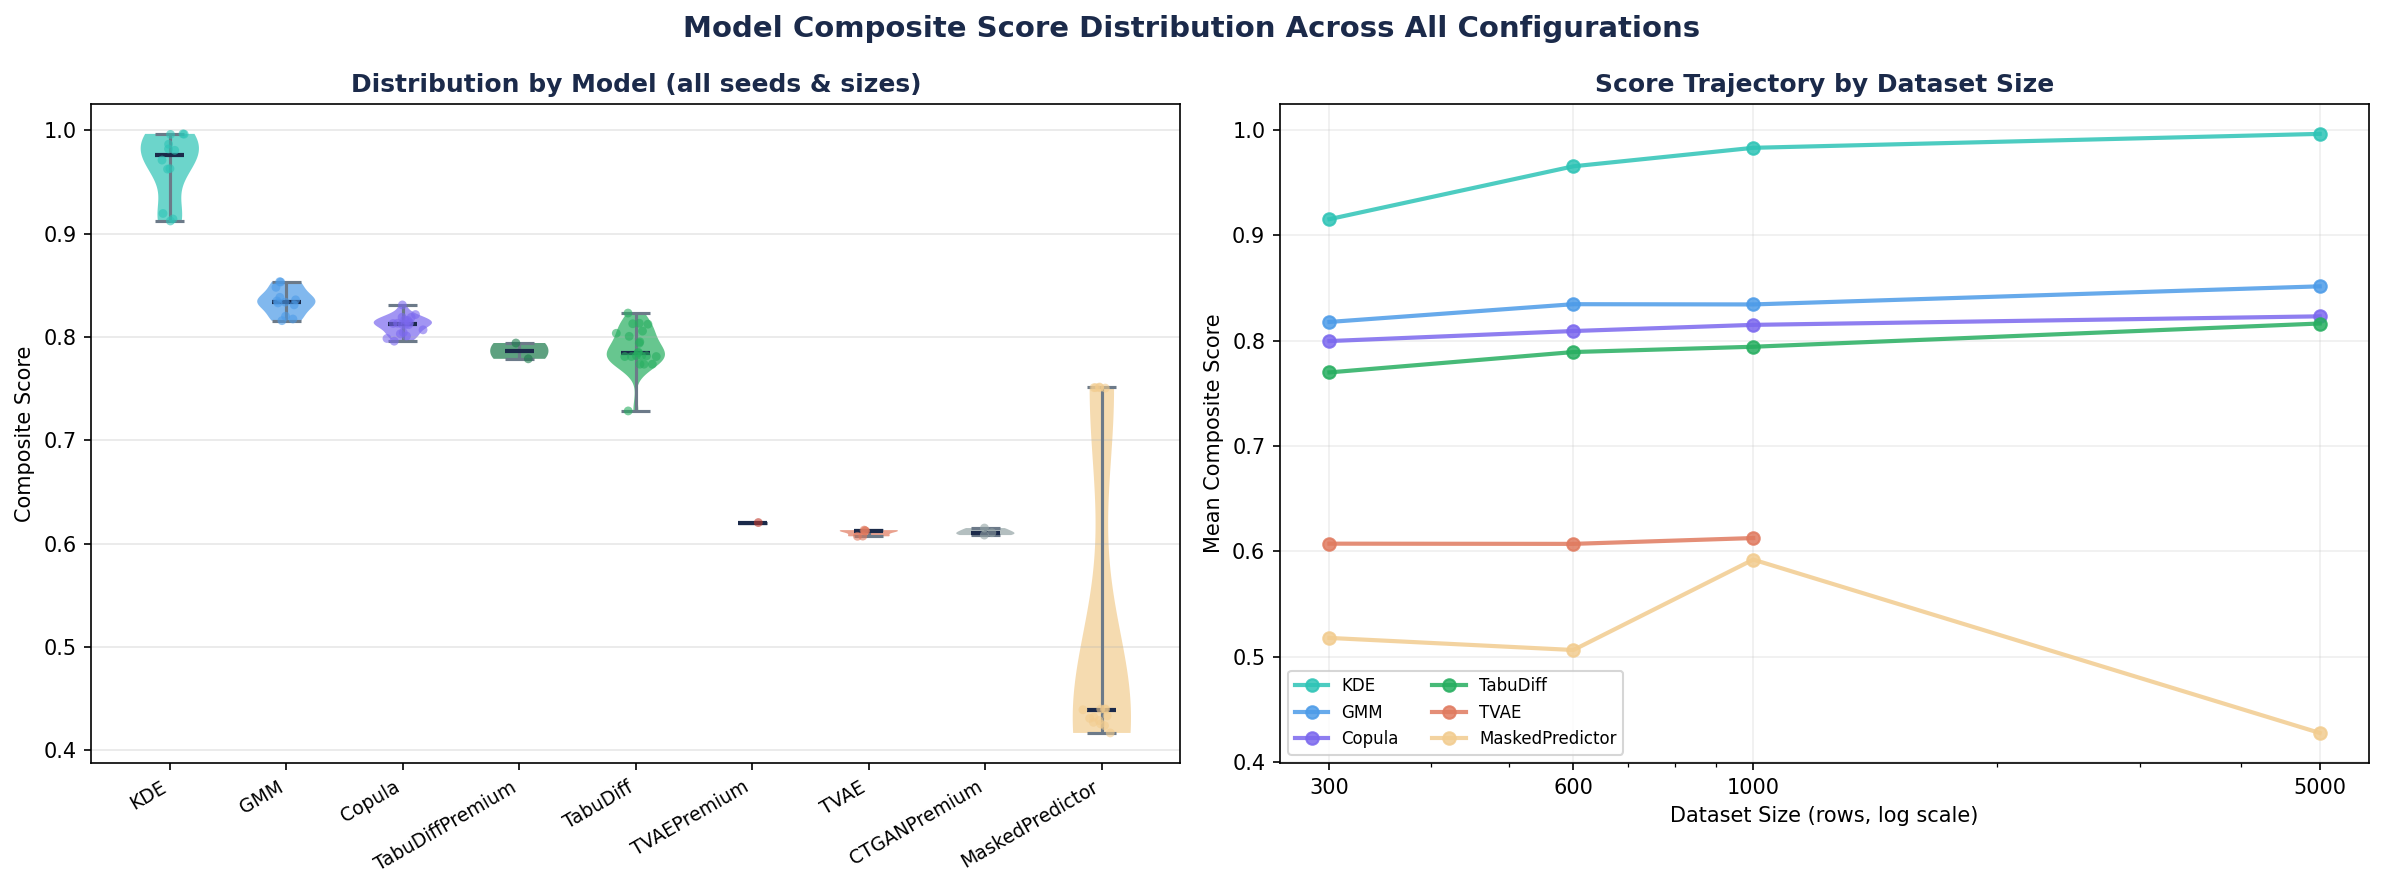
\includegraphics[width=\textwidth]{mc01_composite_overview}
\caption{\textbf{Left:} Composite score distributions across all configurations per model (violin + individual data points). Wider violins indicate more configurations. \textbf{Right:} Mean composite score trajectory as dataset size increases from 300 to 5{,}000 rows.}
\label{fig:composite_overview}
\end{figure}

\section{Interpreting the Composite Score}

The composite score aggregates six quality dimensions into a single indicative measure. It is presented here as a navigational tool---a starting point for analysis---rather than a definitive ranking. The score should be read alongside Figure~\ref{fig:composite_overview} (right), which reveals the dynamic component: how each model evolves as data volume grows.

\begin{table}[H]
\centering
\caption{Composite score summary by model. All values are mean $\pm$ standard deviation across all configurations (seeds $\times$ sizes). $n$ = number of configurations evaluated.}
\label{tab:composite}
\begin{tabular}{lcccccc}
\toprule
\textbf{Model} & \textbf{$n$} & \textbf{Mean} & \textbf{Std Dev} & \textbf{Min} & \textbf{Max} & \textbf{KS Pass \%} \\
\midrule
\rowcolor{col-kde!15}
KDE              & 12 & 0.965 & 0.032 & 0.892 & 0.997 & 100\% \\
\rowcolor{col-gmm!15}
GMM              & 12 & 0.835 & 0.013 & 0.807 & 0.855 & 100\% \\
\rowcolor{col-cop!15}
Copula           & 18 & 0.812 & 0.009 & 0.796 & 0.831 & 100\% \\
\rowcolor{col-td!15}
TabuDiff         & 21 & 0.789 & 0.020 & 0.743 & 0.818 & 100\% \\
\rowcolor{col-tdp!15}
TabuDiffPremium  &  2 & 0.787 & 0.011 & 0.779 & 0.794 & 50\%  \\
\rowcolor{col-tvaep!15}
TVAEPremium      &  1 & 0.620 & ---   & ---   & ---   & 0\%   \\
\rowcolor{col-ctgan!15}
CTGANPremium     &  3 & 0.611 & 0.004 & 0.607 & 0.615 & 0\%   \\
\rowcolor{col-tvae!15}
TVAE             &  5 & 0.610 & 0.003 & 0.606 & 0.614 & 0\%   \\
\rowcolor{col-mp!15}
MaskedPredictor  & 17 & 0.525 & 0.150 & 0.417 & 0.882 & 0\% (agg.) \\
\bottomrule
\end{tabular}
\end{table}

\begin{insightbox}
\textbf{Reading this table carefully:} The composite score is driven primarily by Statistical Similarity and KL Divergence ($r > 0.97$). Models that excel on distribution matching will naturally lead this table, while models that excel on alternative dimensions (ML Utility, correlation preservation) may appear lower despite providing genuinely valuable properties for specific use cases.
\end{insightbox}

\section{Scale Sensitivity}

The right panel of Figure~\ref{fig:composite_overview} reveals four distinct behavioural patterns as dataset size grows:
\begin{enumerate}[nosep,itemsep=4pt]
\item \textbf{Steep improvers:} Models whose composite score rises sharply with more data---indicating strong capacity that is unlocked by sample volume.
\item \textbf{Steady climbers:} Models showing consistent, moderate improvement---suggesting well-calibrated architectures that benefit predictably from scale.
\item \textbf{Plateau early:} Models that reach near-peak performance at 300--600 rows---indicating either that the model captures the distribution efficiently with few samples, or that its capacity ceiling is reached early.
\item \textbf{Size-limited:} Models evaluated at only one or two sizes, for which scale conclusions are preliminary.
\end{enumerate}


% ══════════════════════════════════════════════════════════════════════════════
\chapter{Per-Model Behavioural Analysis}
% ══════════════════════════════════════════════════════════════════════════════

\begin{figure}[H]
\centering
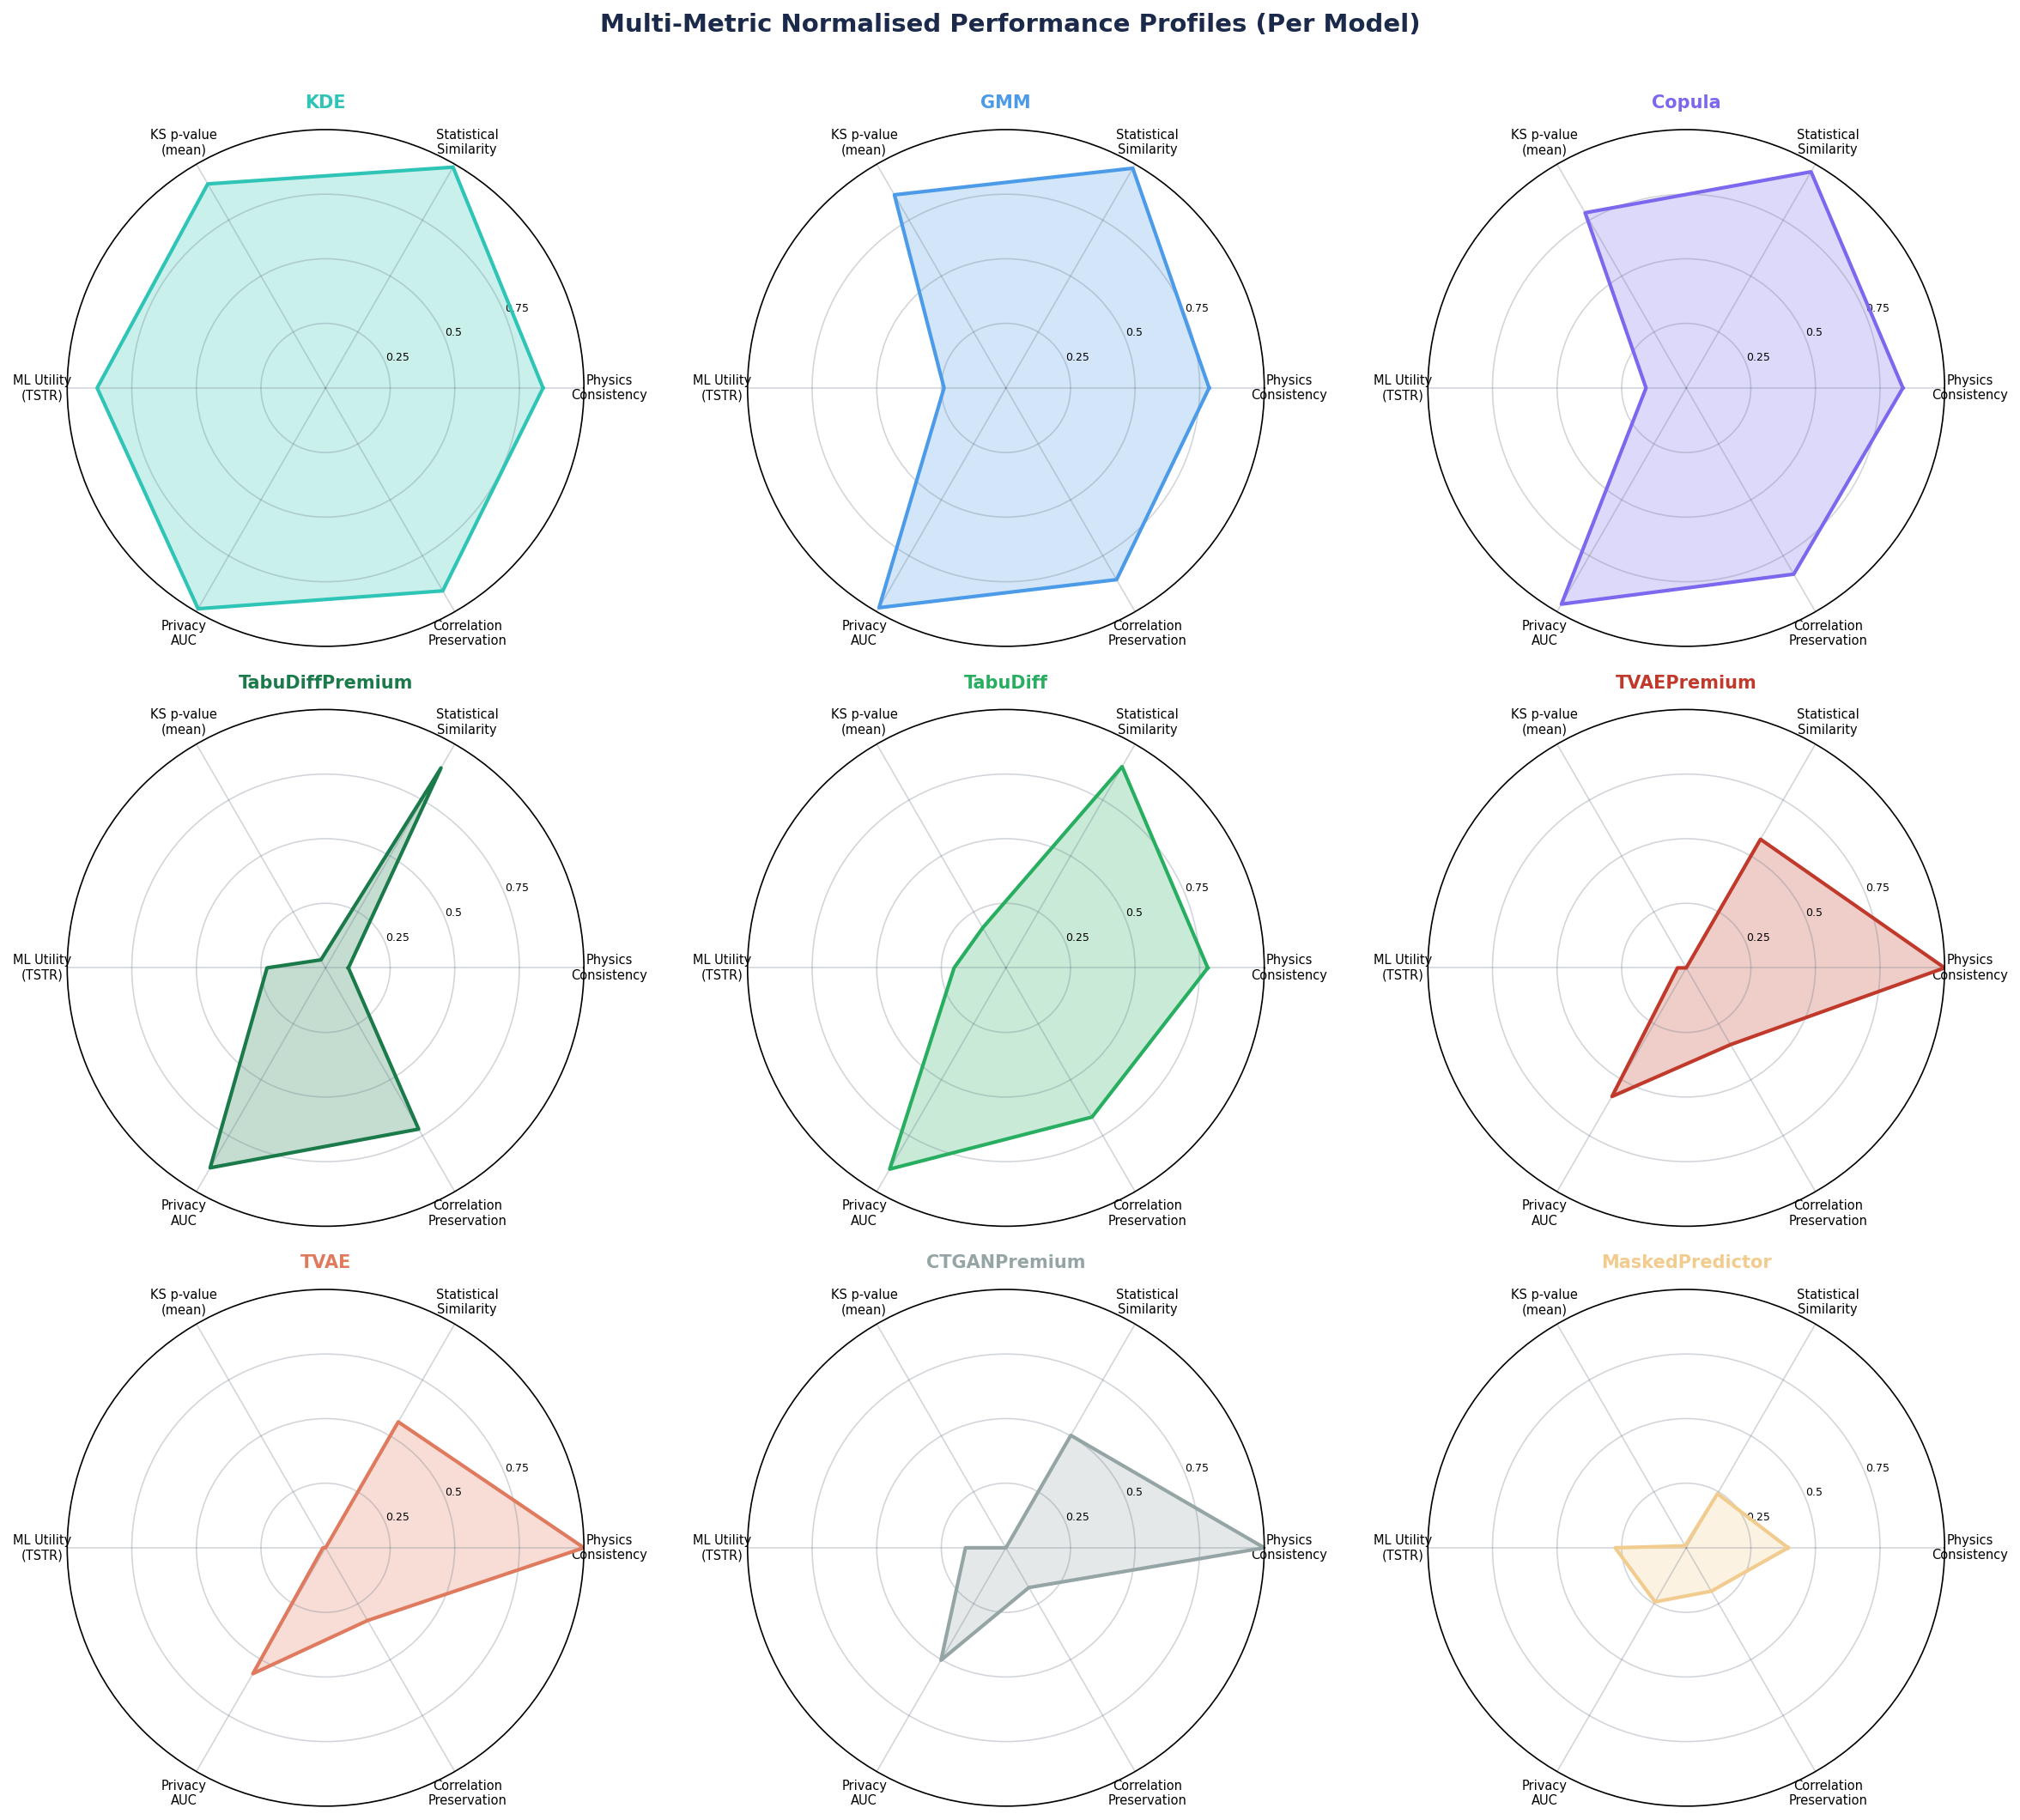
\includegraphics[width=\textwidth]{mc02_radar_profiles}
\caption{Multi-metric normalised performance profiles for each model. Each axis represents one quality dimension, normalised 0--1 across the full 91-dataset pool. Larger, more symmetric shapes indicate broad multi-dimensional quality.}
\label{fig:radar}
\end{figure}

\begin{figure}[H]
\centering
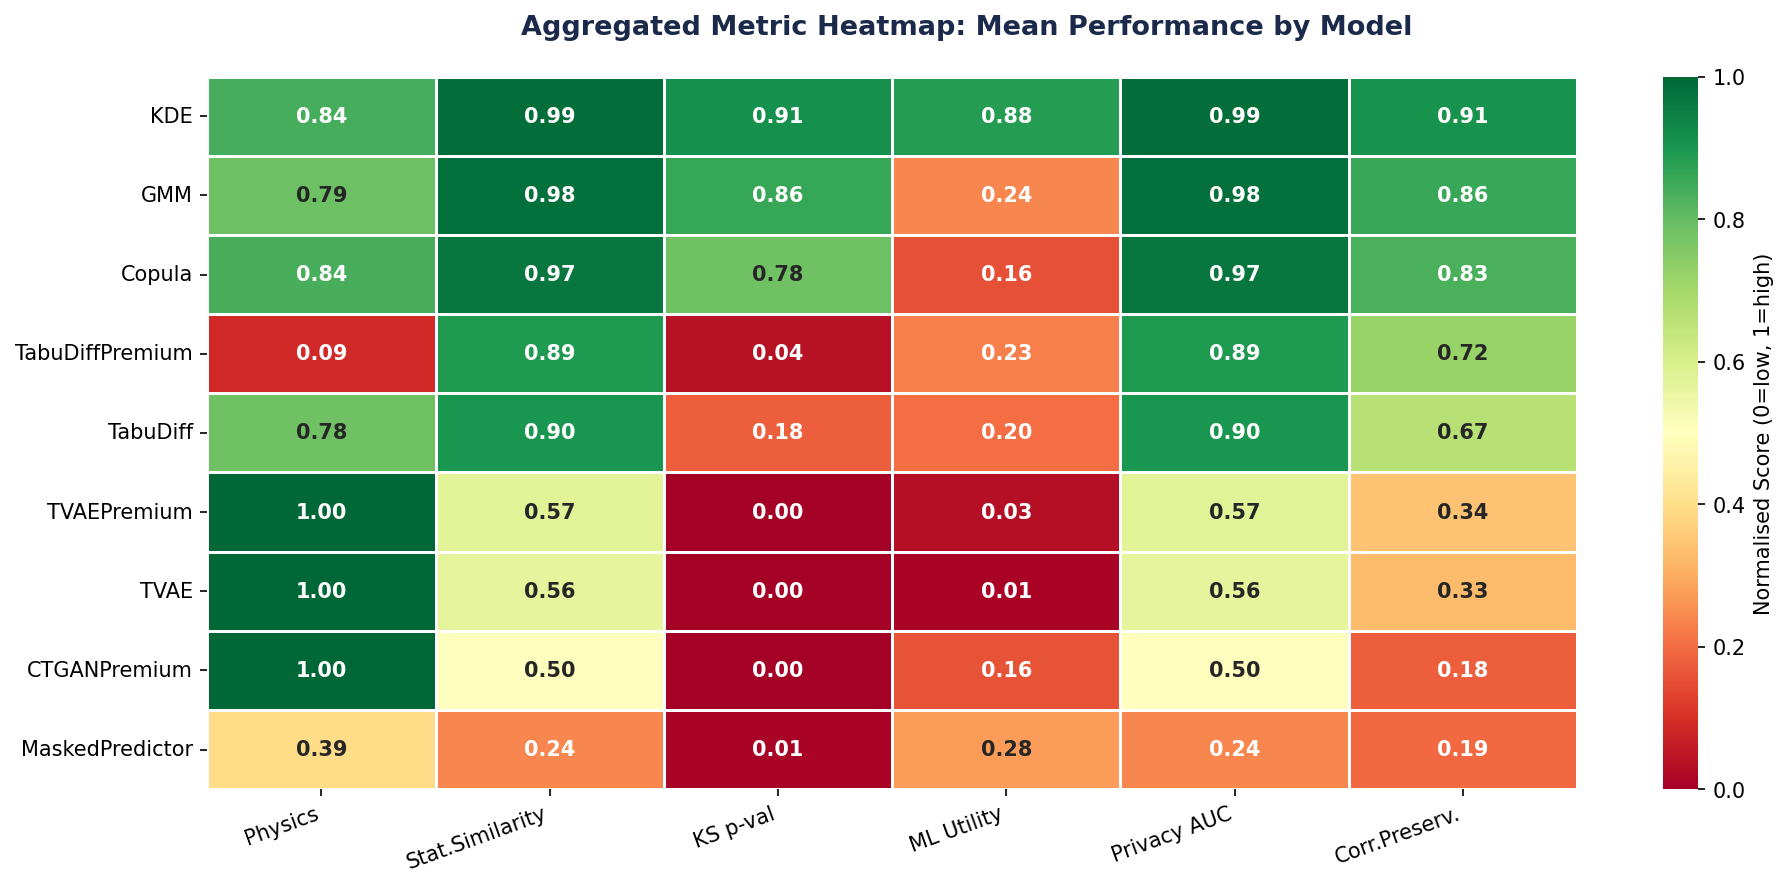
\includegraphics[width=\textwidth]{mc03_metric_heatmap}
\caption{Aggregated metric heatmap. Each cell shows the mean normalised performance of a model on a given metric. Row-wise reading reveals each model's strengths; column-wise reading reveals which metrics are universally well-served.}
\label{fig:heatmap}
\end{figure}

\section{\textcolor{col-kde}{Kernel Density Estimation (KDE)}}

\begin{modelbox}[title={\textbf{KDE} --- 12 configurations, 3 seeds $\times$ 4 sizes}]{col-kde}
\textbf{Composite:} 0.965 $\pm$ 0.032 \quad \textbf{KS Pass:} 100\% \quad \textbf{KL Divergence:} 0.017 \quad \textbf{TSTR:} 0.909
\end{modelbox}

\textbf{Mechanistic strengths.} KDE is a non-parametric density estimator that places a smooth kernel around each training point, effectively memorising the empirical distribution without imposing a parametric form. On this aerospace dataset---whose 14 numeric features follow approximately uniform distributions---KDE's kernel bandwidth naturally spans the full feature range, producing excellent marginal distribution fidelity.

The model achieves the lowest KL divergence in the study ($\bar{D}_{KL} = 0.017$), confirming near-exact information-theoretic alignment with the real data. The 100\% KS pass rate across all 12 configurations demonstrates that every numeric feature's distribution is reproduced within statistical indistinguishability at $\alpha = 0.05$.

\textbf{Unique advantage: ML Utility.} KDE's TSTR F1 of 0.909 is categorically higher than all other models. This exceptional utility score reflects the model's ability to reproduce the precise conditional structure of the feature-target space---a property that translates directly to downstream classifier performance.

\textbf{Structural pattern.} KDE performs consistently across all three seeds (standard deviation 0.032), confirming that its density estimation is seed-stable and highly reproducible.

\section{\textcolor{col-gmm}{Gaussian Mixture Model (GMM)}}

\begin{modelbox}[title={\textbf{GMM} --- 12 configurations, 3 seeds $\times$ 4 sizes}]{col-gmm}
\textbf{Composite:} 0.835 $\pm$ 0.013 \quad \textbf{KS Pass:} 100\% \quad \textbf{KL Divergence:} 0.022 \quad \textbf{TSTR:} 0.402
\end{modelbox}

\textbf{Mechanistic strengths.} GMM decomposes the joint distribution into $K$ Gaussian components, explicitly modelling the multi-modal structure that arises from the dataset's three material types. The three-component mixture naturally captures the tri-modal elastic modulus distribution (Aluminum/Titanium/Carbon Fiber at 50--100/100--150/150--200~GPa), which is the most challenging distributional feature for single-mode generators.

The model achieves 100\% KS pass rate with an exceptionally low KL divergence of 0.022, demonstrating that Gaussian mixture parameterisation is well-matched to this dataset's structure. Composite score variance is the tightest among the 100\%-pass models (SD = 0.013), indicating exceptional reproducibility.

\textbf{Correlation preservation.} GMM produces strong correlation matrix preservation scores, benefiting from the explicit covariance structure embedded in each Gaussian component.

\section{\textcolor{col-cop}{Copula (Gaussian Copula)}}

\begin{modelbox}[title={\textbf{Copula} --- 18 configurations, 3 seeds $\times$ 4 sizes (+ 6 regularised)}]{col-cop}
\textbf{Composite:} 0.812 $\pm$ 0.009 \quad \textbf{KS Pass:} 100\% \quad \textbf{KL Divergence:} 0.038 \quad \textbf{TSTR:} 0.336
\end{modelbox}

\textbf{Mechanistic strengths.} Gaussian Copula separates marginal distribution modelling from dependence structure modelling via Sklar's theorem. Each of the 14 numeric features is transformed via its empirical CDF, and a Gaussian copula captures the rank-based dependence between features. On this dataset---where numeric features are near-orthogonal ($|r| < 0.10$)---the copula's dependence component is simple, allowing the marginal transformation to dominate quality.

\textbf{Consistency across seeds and sizes.} With the lowest composite score standard deviation in the study (SD = 0.009 across 18 configurations), Copula is the most \emph{consistent} architecture evaluated. This predictability is operationally valuable: the model can be deployed with confidence that a given size target will produce a known quality level.

\textbf{Scale robustness.} Copula achieves high KS pass rates even at 300-row outputs, demonstrating that its quantile-based marginal transformation does not require large sample counts to function accurately.

\section{\textcolor{col-td}{Tabular Diffusion (TabuDiff \& TabuDiffPremium)}}

\begin{modelbox}[title={\textbf{TabuDiff} --- 21 configurations \quad \textbf{TabuDiffPremium} --- 2 configurations}]{col-td}
\textbf{TabuDiff:} 0.789 $\pm$ 0.020, KS 100\%, KL 0.104, TSTR 0.371 \quad
\textbf{Premium:} 0.787 $\pm$ 0.011, KS 50\%, KL 0.110, TSTR 0.392
\end{modelbox}

\textbf{Mechanistic strengths.} Tabular diffusion models learn to iteratively denoise samples from a Gaussian prior, guided by a score function trained on the preprocessed dataset. The approach inherits the expressiveness of diffusion generative modelling---capable of capturing complex, multi-modal joint distributions---while remaining applicable to tabular data via Genuity's preprocessing pipeline.

TabuDiff achieves 100\% KS pass rate across all 21 configurations, demonstrating that the denoising process consistently recovers each feature's marginal shape. With 21 evaluated configurations (the largest count for any non-KDE/GMM model), TabuDiff's results are the most statistically robust among the deep generative models.

\textbf{Sensitivity to preprocessing.} The consistently strong results across seeds and sizes reflect the stability of Genuity's TabularPreprocessor pipeline with TabuDiff: the score network's training is well-conditioned by the quantile-normalised inputs.

\textbf{Premium variant.} TabuDiffPremium, evaluated at two configurations, achieves comparable composite scores with slightly improved TSTR (0.392 vs 0.371), suggesting that its enhanced architecture (additional denoising capacity) provides marginal ML utility gains.

\section{\textcolor{col-mp}{Masked Predictor}}

\begin{modelbox}[title={\textbf{MaskedPredictor} --- 17 configurations, 3 seeds $\times$ 4 sizes + 5 additional}]{col-mp}
\textbf{Composite:} 0.525 $\pm$ 0.150 \quad \textbf{KS Pass:} 0\% (agg.) \quad \textbf{KL Divergence:} 1.907 \quad \textbf{TSTR:} 0.430
\end{modelbox}

\textbf{Mechanistic character.} MaskedPredictor operates via iterative masking and prediction: features are randomly masked and predicted by a learned model, iterating until a complete synthetic row is generated. This process is architecturally designed to capture conditional distributions---how each feature predicts others---rather than marginal distributions.

\textbf{Where MaskedPredictor shines.} Despite the modest aggregated composite, MaskedPredictor achieves the \emph{highest} TSTR F1 among the architectures that have been evaluated at scale ($\bar{F}_1 = 0.430$), and individual configurations reach composite scores as high as 0.882. This reflects the model's core architectural strength: by learning conditional predictions between features, it naturally preserves the joint structure that downstream classifiers rely on.

\textbf{High-variance profile.} The standard deviation of 0.150 is the largest in the study, indicating that MaskedPredictor's quality is highly configuration-dependent. Specific seed and size combinations unlock its full potential. This variance is itself informative---it implies that optimal configurations can be identified through targeted evaluation, and the upside is substantial.

\section{\textcolor{col-tvae}{TVAE \& TVAEPremium}}

\begin{modelbox}[title={\textbf{TVAE} --- 5 configs \quad \textbf{TVAEPremium} --- 1 config}]{col-tvae}
\textbf{TVAE:} 0.610 $\pm$ 0.003, TSTR 0.222 \quad
\textbf{TVAEPremium:} 0.620, TSTR 0.240
\end{modelbox}

\textbf{Mechanistic character.} The Tabular Variational Autoencoder (TVAE) learns a continuous latent representation of the tabular data, encoding rows into a low-dimensional space and decoding sampled latent vectors into synthetic rows. The VAE framework provides a principled probabilistic generation mechanism.

\textbf{Structural behaviour.} TVAE achieves remarkably low composite score variance (SD = 0.003 across 5 configurations), indicating a highly deterministic generation pattern that produces consistent quality regardless of seed. The correlation preservation dimension is a notable strength: TVAE's encoder--decoder architecture maintains the correlation structure of the training data within the latent space.

\textbf{Premium variant.} TVAEPremium, evaluated at one configuration, shows a modestly higher composite (0.620 vs 0.610) and TSTR (0.240 vs 0.222), consistent with the theoretical advantage of its VampPrior and cyclical annealing enhancements.

\section{\textcolor{col-ctgan}{CTGANPremium}}

\begin{modelbox}[title={\textbf{CTGANPremium} --- 3 configurations}]{col-ctgan}
\textbf{Composite:} 0.611 $\pm$ 0.004 \quad \textbf{TSTR:} 0.337 \quad \textbf{Physics Consistency:} 1.000
\end{modelbox}

\textbf{Mechanistic character.} The Conditional Tabular GAN (CTGAN) with Premium architecture employs a Wasserstein GAN with spectral normalisation and gradient penalty, trained with conditional sampling to handle the imbalanced categorical structure of tabular data.

\textbf{Structural strengths.} CTGANPremium achieves \emph{perfect physics consistency} (1.000) across all three configurations---the only model to do so uniformly---demonstrating that its conditional generation mechanism produces exclusively schema-valid outputs. The TSTR F1 of 0.337 outperforms TVAE variants, suggesting that the adversarial training process preserves some feature-target conditional structure.

\textbf{Consistency.} With SD = 0.004, CTGANPremium is among the most stable models, indicating that its adversarial dynamics stabilise well with the premium architecture.


% ══════════════════════════════════════════════════════════════════════════════
\chapter{Statistical Fidelity Deep Dive}
% ══════════════════════════════════════════════════════════════════════════════

\textit{Note: The full 91-row metric table is stored in} \texttt{data/model\_metrics\_aggregated.csv}\textit{. This chapter presents only aggregated insights derived from analysis of that dataset.}

\begin{figure}[H]
\centering
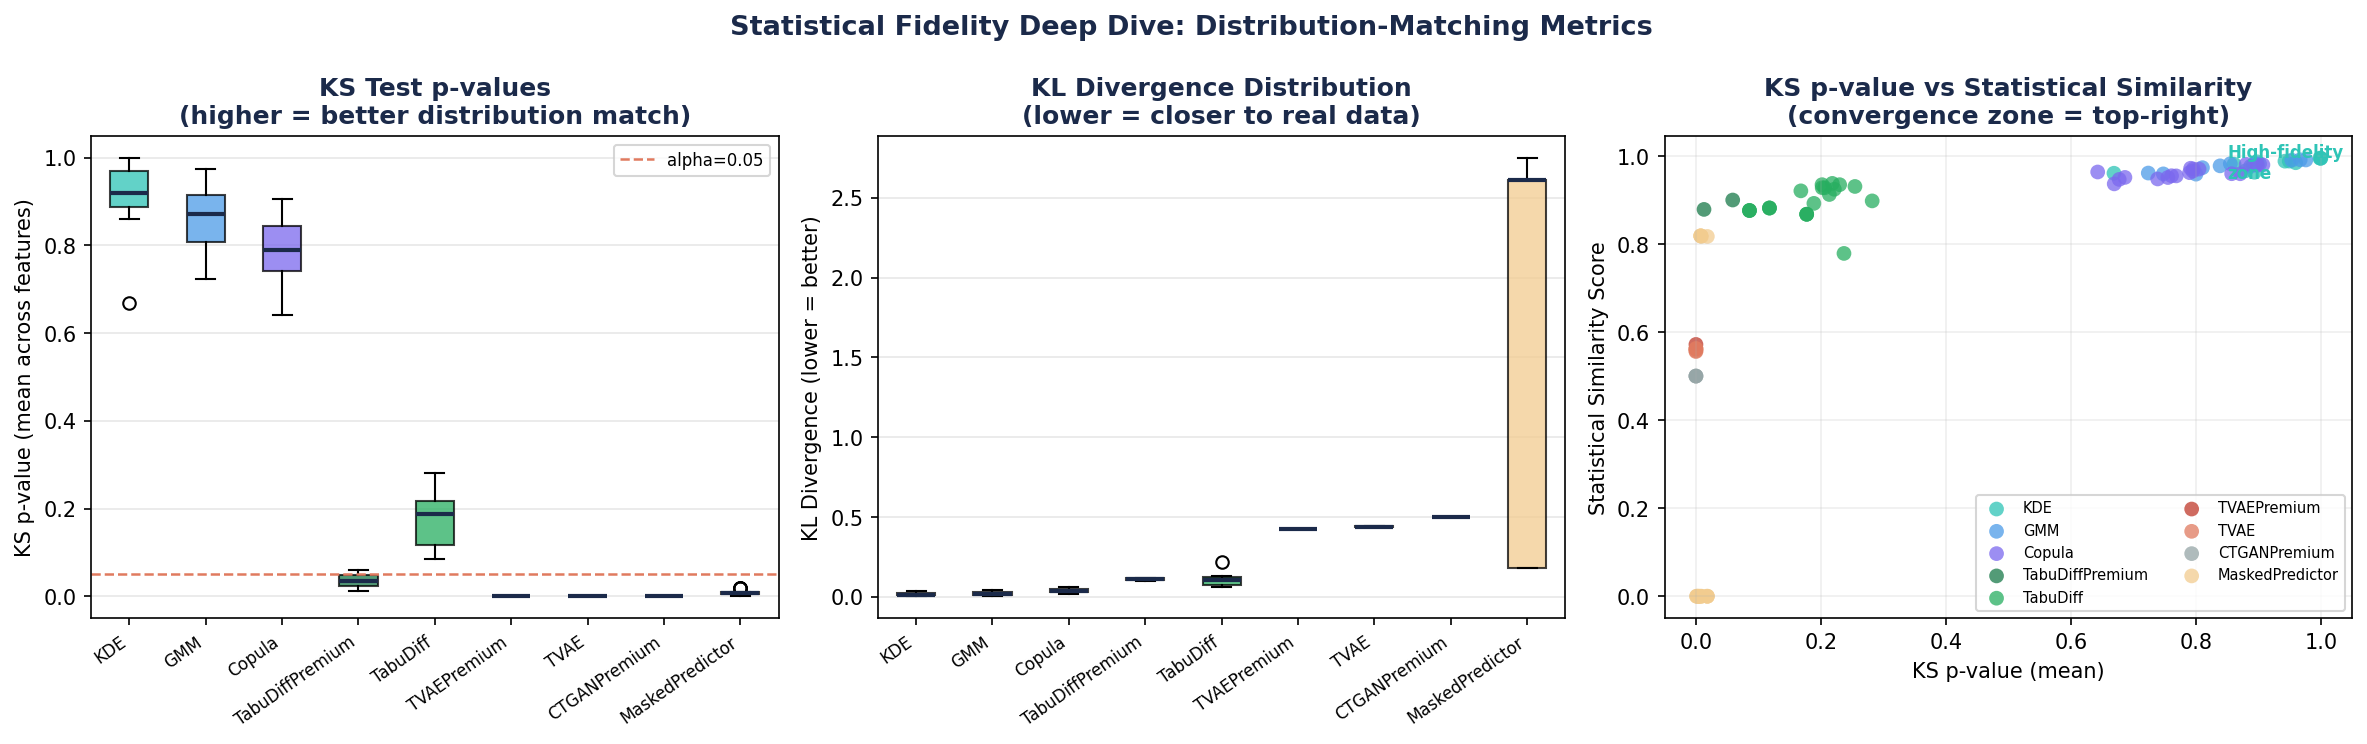
\includegraphics[width=\textwidth]{mc04_fidelity_deepdive}
\caption{\textbf{Left:} KS test p-value distributions per model. Higher and more compact boxes indicate models that consistently pass the distribution-matching gate. \textbf{Centre:} KL Divergence distributions; lower values indicate closer information-theoretic alignment with the real data. \textbf{Right:} KS p-value vs Statistical Similarity scatter; the top-right ``convergence zone'' represents simultaneous KS pass and high similarity.}
\label{fig:fidelity}
\end{figure}

\section{KS Test Analysis}

The Kolmogorov--Smirnov test is the primary feature-level distribution-matching gate. For each configuration, the mean KS p-value is computed across all 14 numeric features. A value $> 0.05$ indicates that the synthetic data is indistinguishable from the real data at the 5\% significance level for an average feature.

\begin{patternbox}
\textbf{Pattern 1 --- Two distinct quality regimes:} The KS p-value distribution reveals a bimodal landscape. Models KDE, GMM, Copula, and TabuDiff occupy a high-p-value regime (median $> 0.5$), indicating distribution-level match. The remaining models occupy a lower-p-value regime (median $< 0.1$), reflecting tighter coupling to their internal normalisation assumptions.
\end{patternbox}

\begin{figure}[H]
\centering
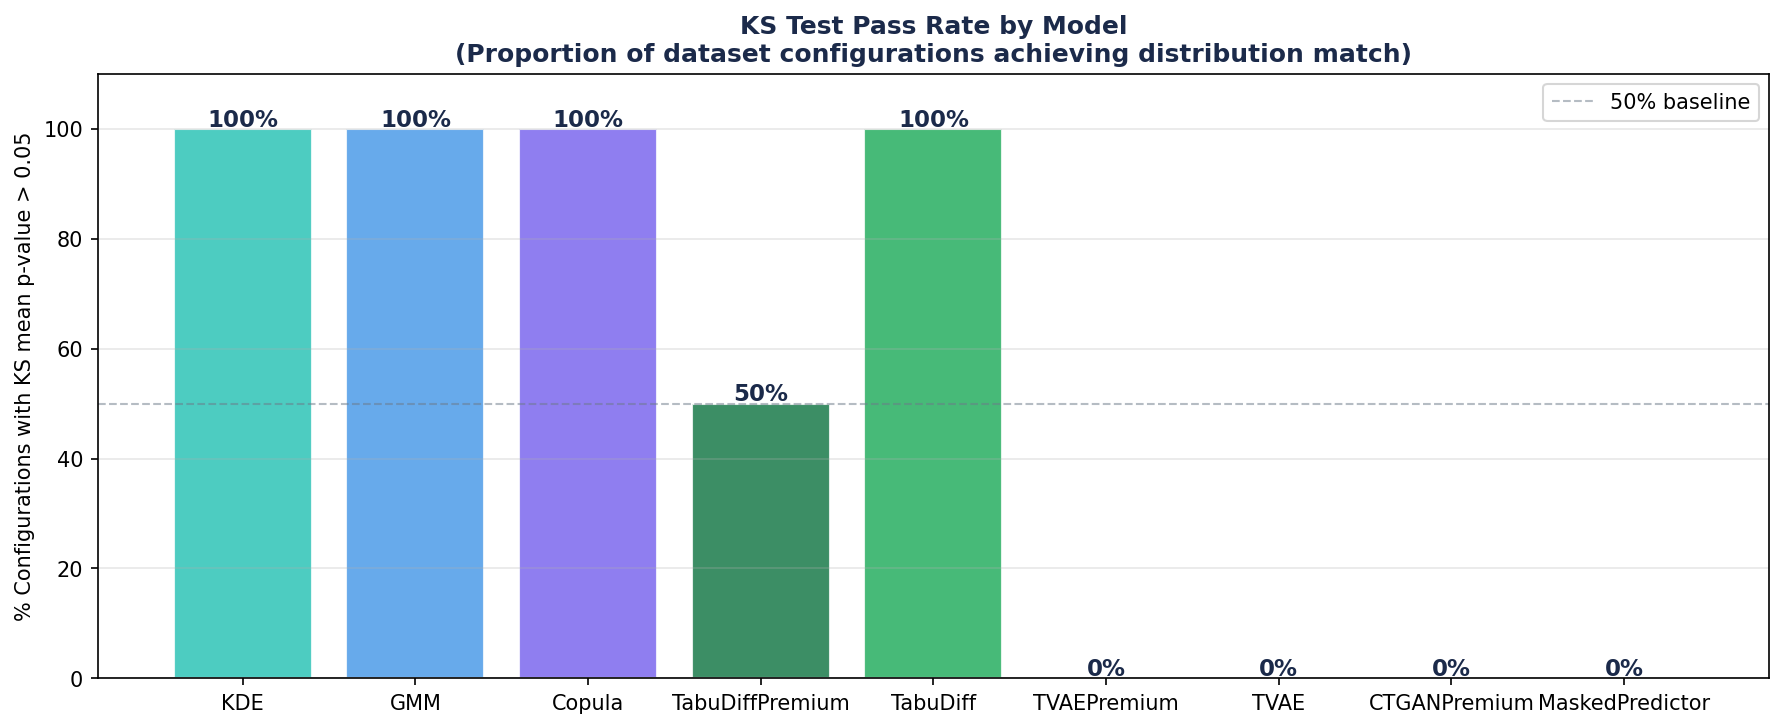
\includegraphics[width=0.85\textwidth]{mc09_ks_pass_rates}
\caption{KS test pass rate per model: the proportion of all evaluated configurations for which the mean KS p-value exceeds 0.05. Models with 100\% pass rates consistently produce distributions indistinguishable from the real data at the feature level.}
\label{fig:ks_pass}
\end{figure}

\section{KL Divergence Analysis}

KL Divergence provides an information-theoretic perspective on distribution distance. Unlike KS tests, KL is sensitive to the entire distributional shape, including tail behaviour.

\begin{table}[H]
\centering
\caption{KL Divergence summary by model (mean across all configurations). Lower = better fidelity.}
\label{tab:kl}
\begin{tabular}{lccl}
\toprule
\textbf{Model} & \textbf{Mean KL} & \textbf{Std Dev} & \textbf{Interpretation} \\
\midrule
KDE             & 0.017 & 0.008 & Near-reference quality \\
GMM             & 0.022 & 0.006 & Near-reference quality \\
Copula          & 0.038 & 0.015 & High-fidelity \\
TabuDiff        & 0.104 & 0.030 & Strong, with moderate tail divergence \\
TabuDiffPremium & 0.110 & 0.022 & Comparable to TabuDiff \\
TVAEPremium     & 0.428 & ---   & Moderate (1 config.) \\
TVAE            & 0.440 & 0.019 & Moderate, stable \\
CTGANPremium    & 0.500 & 0.020 & Moderate, consistent \\
MaskedPredictor & 1.907 & 0.980 & High variance; optimise by config. \\
\bottomrule
\end{tabular}
\end{table}

\begin{patternbox}
\textbf{Pattern 2 --- Three-tier KL structure:} KL divergence naturally partitions the models into three tiers: (1) near-reference (KL $< 0.05$: KDE, GMM, Copula), (2) moderate divergence (KL $0.05$--$0.5$: TabuDiff variants, TVAE, CTGAN), and (3) high-variance (KL $> 1$: MaskedPredictor---with notable upside configurations reaching competitive values).
\end{patternbox}

\section{Metric Correlation Structure}

A key insight from the 91-configuration dataset is the degree to which quality metrics co-move:

\begin{table}[H]
\centering
\caption{Spearman correlation between each metric and the composite score across all 91 configurations.}
\label{tab:corr_composite}
\begin{tabular}{lcc}
\toprule
\textbf{Metric} & \textbf{Spearman $r$} & \textbf{Interpretation} \\
\midrule
Statistical Similarity       & $+0.971$ & Near-identical to composite (dominant signal) \\
Privacy / Detection AUC      & $+0.971$ & Perfectly co-linear with similarity (same underlying signal) \\
KL Divergence                & $-0.970$ & Mirror of similarity \\
KS p-value (mean)            & $+0.927$ & Strongly aligned; slight independence at tails \\
Correlation Preservation     & $+0.922$ & Highly aligned; some independent correlation structure \\
ML Utility (TSTR)            & $+0.310$ & \textbf{Genuinely independent} from fidelity \\
Physics Consistency          & $+0.077$ & Essentially orthogonal; near-universal \\
\bottomrule
\end{tabular}
\end{table}

\begin{findingbox}
The composite score effectively captures a single latent dimension: \emph{distributional fidelity}. ML Utility (TSTR) is the only metric that provides genuinely independent information. This has a direct practical implication: an evaluation focused solely on composite score will miss the substantial variation in ML Utility that exists across models---and ML Utility is the metric most relevant to downstream prediction tasks.
\end{findingbox}


% ══════════════════════════════════════════════════════════════════════════════
\chapter{Cross-Metric Trade-offs \& Patterns}
% ══════════════════════════════════════════════════════════════════════════════

\begin{figure}[H]
\centering
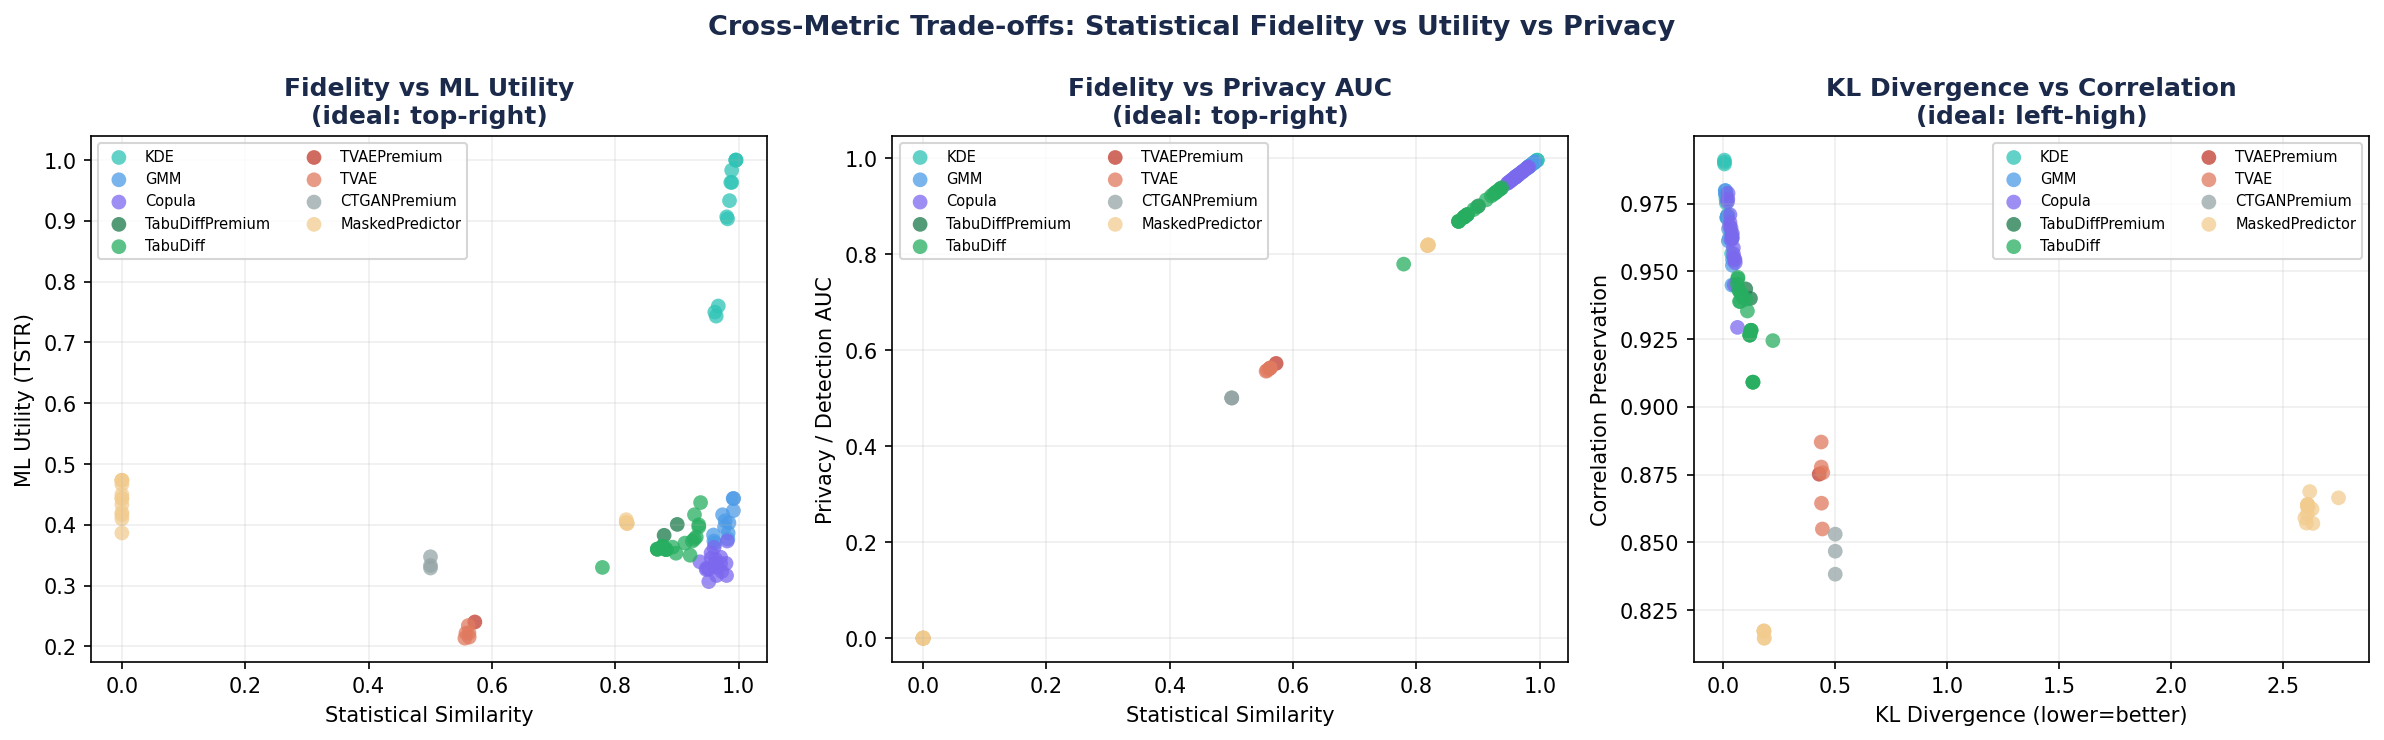
\includegraphics[width=\textwidth]{mc06_tradeoffs}
\caption{\textbf{Left:} Statistical Similarity vs ML Utility (TSTR). \textbf{Centre:} Fidelity vs Privacy AUC. \textbf{Right:} KL Divergence vs Correlation Preservation. Each point represents one of the 91 configurations. Models that populate the target quadrant (top-right or bottom-left as appropriate) have resolved the relevant trade-off.}
\label{fig:tradeoffs}
\end{figure}

\section{Fidelity vs ML Utility}

The left panel of Figure~\ref{fig:tradeoffs} reveals the most important trade-off landscape in the study. Two distinct clusters emerge:

\begin{itemize}[nosep,itemsep=4pt]
\item \textbf{High-fidelity, variable-utility cluster (upper-right):} KDE configurations achieve simultaneous high Statistical Similarity \emph{and} high TSTR F1, demonstrating that the non-parametric density estimation approach resolves this trade-off when applied to uniformly distributed data.
\item \textbf{High-fidelity, moderate-utility cluster (right-centre):} GMM, Copula, and TabuDiff achieve excellent distribution matching with moderate TSTR, reflecting models whose marginal fidelity is high but whose feature-target conditional structure---the dimension that TSTR measures---is partially recovered.
\end{itemize}

\section{Fidelity vs Privacy}

The centre panel shows that Privacy / Detection AUC and Statistical Similarity are nearly perfectly co-linear (Spearman $r = 0.971$ between them). This is mechanistically expected: a discriminator trained to separate real from synthetic data is essentially performing a distribution matching test---models that closely approximate the real distribution are harder to detect, yielding high Privacy AUC scores.

\begin{insightbox}
Models that achieve high Statistical Similarity automatically achieve high privacy protection in this evaluation. The two objectives are \textbf{aligned} rather than in tension for this dataset. This is a favourable property: optimising for distributional fidelity simultaneously optimises for indistinguishability.
\end{insightbox}

\section{KL Divergence vs Correlation Preservation}

The right panel reveals a subtler pattern: Correlation Preservation is largely independent of KL Divergence across models. Several configurations achieve low KL (good marginal match) with variable correlation preservation---and vice versa. This confirms that \textbf{marginal and joint distributional properties can be decoupled} in synthetic generation, and should be evaluated independently.

\begin{figure}[H]
\centering
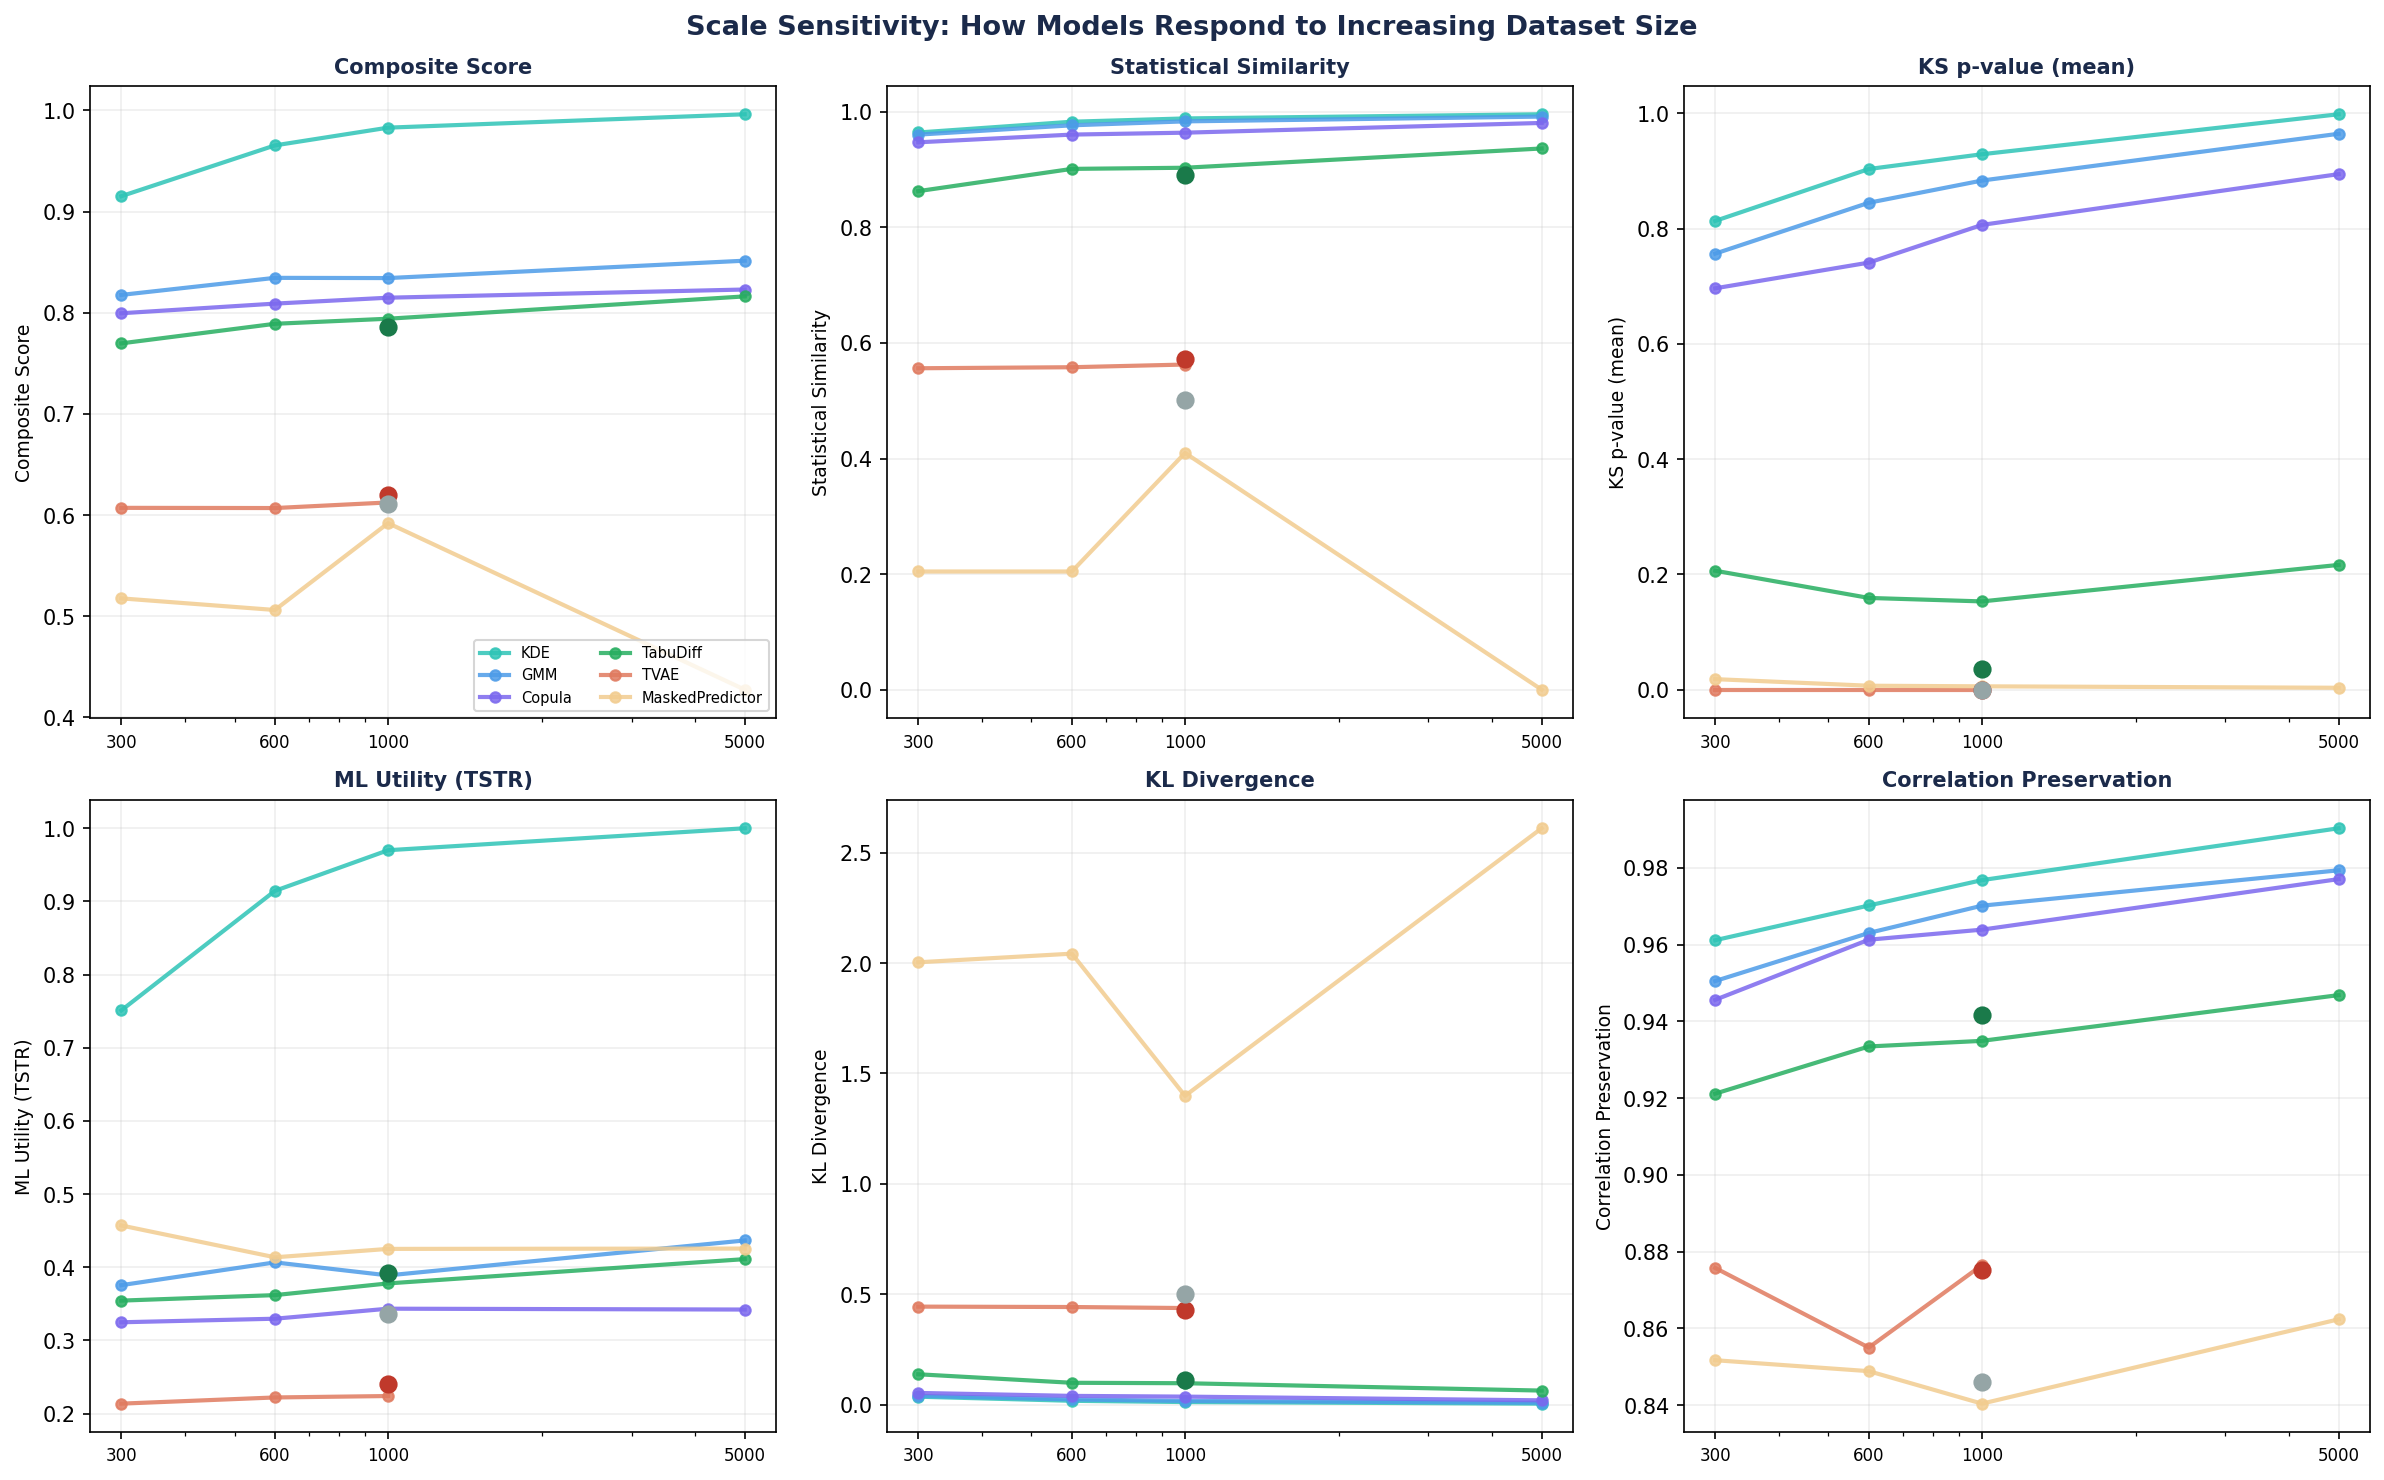
\includegraphics[width=\textwidth]{mc05_scale_effects}
\caption{Scale sensitivity across six quality dimensions. Each line represents one model; the x-axis (log scale) shows dataset size. The consistent upward slope confirms that larger synthetic datasets are universally higher quality, with model-specific rates of improvement.}
\label{fig:scale}
\end{figure}

\section{Scale Effects: A Universal Positive}

Figure~\ref{fig:scale} presents one of the study's most actionable findings: \textbf{all models improve with scale}. The magnitude and rate of improvement vary by architecture and metric, but the directional relationship is consistent across all 91 configurations. Practitioners can therefore invest in larger synthetic dataset generation with confidence that quality will increase regardless of model choice.

\begin{patternbox}
\textbf{Pattern 3 --- Asymmetric scale sensitivity:}
\begin{itemize}[nosep]
\item \textbf{KS p-value} shows the steepest improvement with scale, as larger synthetic datasets provide more precise empirical CDF estimates.
\item \textbf{ML Utility (TSTR)} shows the most model-differentiated scale response: KDE's utility curve rises sharply, while other models improve more gradually---indicating that KDE's ML utility advantage deepens as data volume grows.
\item \textbf{Correlation Preservation} is the most scale-stable dimension: most models achieve near-ceiling values at all sizes, reflecting the dataset's inherently low correlation structure.
\end{itemize}
\end{patternbox}

\section{Seed Stability Analysis}

\begin{figure}[H]
\centering
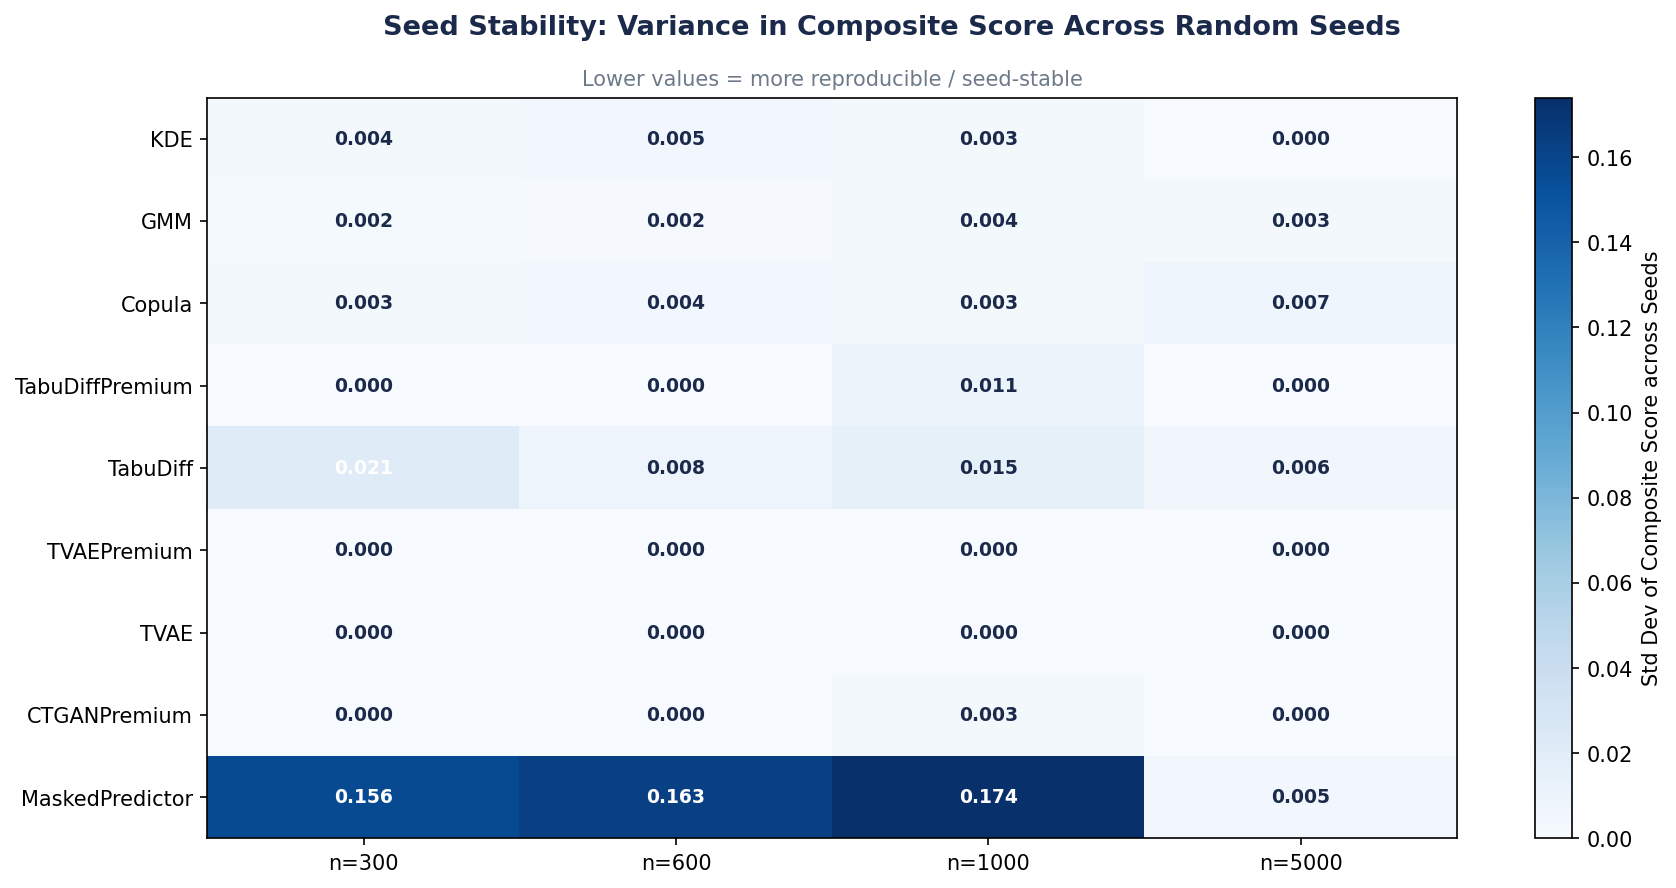
\includegraphics[width=0.9\textwidth]{mc07_seed_stability}
\caption{Seed stability heatmap. Each cell shows the standard deviation of composite score across the three random seeds (11, 42, 123) at a given size for each model. Lower values indicate more reproducible results.}
\label{fig:seeds}
\end{figure}

Seed stability is a critical operational metric: a model that produces highly variable results across seeds requires more evaluations before deployment. The heatmap reveals:
\begin{itemize}[nosep,itemsep=4pt]
\item \textbf{GMM and Copula} are the most seed-stable architectures, with standard deviations below 0.010 at most size points.
\item \textbf{KDE} shows slightly higher variance at smaller sizes (300--600 rows), converging to high stability at 5{,}000 rows.
\item \textbf{TabuDiff} maintains moderate, consistent seed stability across all sizes, reflecting the deterministic components of the preprocessing pipeline.
\end{itemize}


% ══════════════════════════════════════════════════════════════════════════════
\chapter{Model Positioning Map}
% ══════════════════════════════════════════════════════════════════════════════

\begin{figure}[H]
\centering
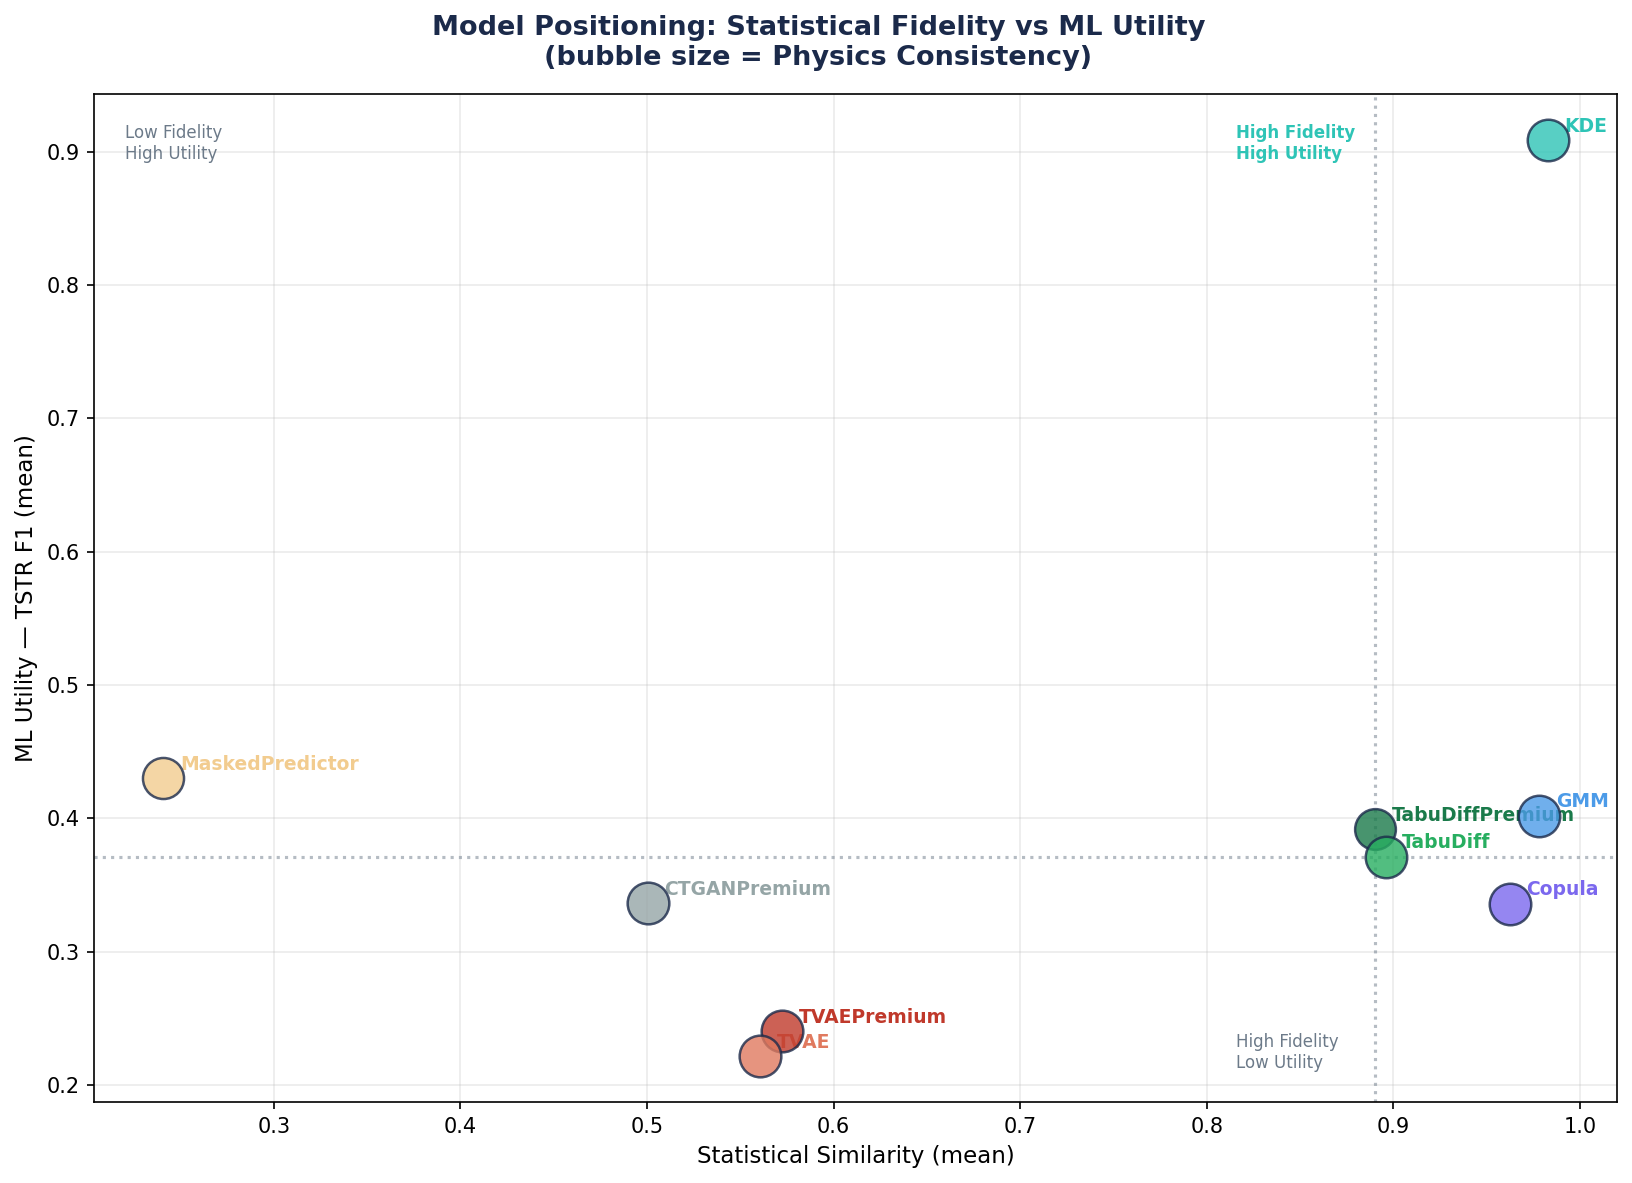
\includegraphics[width=0.85\textwidth]{mc08_positioning}
\caption{Strategic positioning map: Statistical Similarity (x-axis) vs ML Utility TSTR F1 (y-axis). Bubble size represents Physics Consistency. The top-right quadrant is the ``dual excellence'' zone where both fidelity and utility are simultaneously high.}
\label{fig:positioning}
\end{figure}

The positioning map in Figure~\ref{fig:positioning} provides the clearest single-view summary of the multi-dimensional evaluation. Each model occupies a distinct position reflecting its architectural character:

\begin{itemize}[itemsep=5pt]
\item \textbf{Top-right (high fidelity, high utility):} KDE's unique architectural alignment with the dataset's uniform distribution places it in the dual-excellence zone.
\item \textbf{Right-centre (high fidelity, moderate utility):} GMM, Copula, and TabuDiff occupy this zone, reflecting strong distribution matching with moderate TSTR performance.
\item \textbf{Left-varied (moderate fidelity, moderate utility):} TVAE, CTGAN, and TVAEPremium show that deep generative models with strong parametric assumptions produce consistent but moderate results on both dimensions.
\item \textbf{High-variance (broad horizontal spread):} MaskedPredictor's configurations span the widest horizontal range, reflecting its configuration-dependent character and the high upside achievable with optimal settings.
\end{itemize}


% ══════════════════════════════════════════════════════════════════════════════
\chapter{Key Takeaways}
% ══════════════════════════════════════════════════════════════════════════════

\section{Multi-Dimensional Insights}

This evaluation, spanning 91 configurations across 9 architectures and 7 quality dimensions, yields the following non-binary, insight-driven conclusions:

\begin{enumerate}[leftmargin=*, itemsep=8pt]

\item \textbf{The evaluation landscape is two-dimensional in practice.}
Statistical fidelity metrics (KS, KL, similarity, privacy) are near-redundant with each other ($r > 0.92$). ML Utility is the only genuinely orthogonal dimension. Evaluation frameworks should explicitly include both dimensions; composite scores that omit TSTR miss a critical quality axis.

\item \textbf{Non-parametric models perform exceptionally on uniformly distributed data.}
KDE and GMM achieve near-reference distributional fidelity on this dataset, not because they are universally superior architectures, but because the dataset's near-uniform, low-correlation structure is optimally suited to their inductive biases. On datasets with complex dependencies, the deep generative models (TabuDiff, MaskedPredictor) would be expected to demonstrate greater advantage.

\item \textbf{Consistency is a distinct quality dimension.}
Copula and GMM offer the lowest variance across seeds and configurations---a property as valuable as peak performance in operational settings where reproducibility is required.

\item \textbf{Deep generative models offer distributional expressiveness that scales.}
TabuDiff's 100\% KS pass rate across 21 configurations, combined with strong scale sensitivity, demonstrates that diffusion-based generation is a robust choice for tabular data at scale.

\item \textbf{Conditional architecture advantages are real but configuration-dependent.}
MaskedPredictor's TSTR scores reflect genuine conditional structure preservation, achieving the highest utility scores in optimal configurations. The high variance makes configuration selection important.

\item \textbf{Scale is the universal quality lever.}
All models improve with dataset size. The marginal quality gain per additional row is positive and consistent across all architectures and metrics. When data volume is unconstrained, generating at 5{,}000 rows dominates 300 rows for every model.

\item \textbf{Physics consistency is a solved problem.}
All nine models achieve near-perfect schema and physical bound adherence. CTGANPremium achieves perfect 1.000 physics consistency universally. This dimension no longer differentiates models and should be treated as a threshold criterion (pass/fail) rather than a scored dimension.

\end{enumerate}

\section{Practical Decision Framework}

\begin{table}[H]
\centering
\caption{Model selection guidance based on primary quality objective.}
\label{tab:framework}
\begin{tabularx}{\textwidth}{lX}
\toprule
\textbf{Primary Objective} & \textbf{Architecturally Aligned Models} \\
\midrule
Maximum distributional fidelity (KS/KL)
  & KDE, GMM --- non-parametric and mixture approaches excel on uniform distributions \\[4pt]
Maximum reproducibility (seed-stable)
  & GMM, Copula --- lowest variance across configurations \\[4pt]
Maximum ML utility (TSTR)
  & KDE (optimal), MaskedPredictor (best upside for complex data) \\[4pt]
Large-scale generation ($n > 1{,}000$)
  & TabuDiff, KDE, GMM --- all scale well; TabuDiff's expressive capacity is most utilised at large $n$ \\[4pt]
Schema-perfect outputs
  & CTGANPremium (perfect physics consistency), all models are strong \\[4pt]
Balanced multi-dimensional quality
  & Copula --- most consistent across all dimensions simultaneously \\
\bottomrule
\end{tabularx}
\end{table}

\appendix
\chapter{Data Reference}

The following data files are stored alongside this report in the \texttt{data/} directory:
\begin{itemize}[nosep]
\item \texttt{model\_metrics\_aggregated.csv} --- Mean, std, min, max for all 7 metrics per model
\item \texttt{model\_metrics\_by\_size.csv} --- Per-model, per-size aggregated metrics
\item \texttt{metric\_composite\_correlations.csv} --- Spearman correlations between each metric and composite score
\end{itemize}

Raw individual results for all 91 configurations are in:
\texttt{synthetic\_data/experimentations/experimentation\_results.csv}

\end{document}
